\section{Вектор}

\subsection{Определение вектора}

\begin{definition}
	\textit{Вектор} $-$ направленный отрезок, концы которого упорядочены.
\end{definition}

Вектор принято обозначать следующим образом:

\begin{itemize}
	\item $\overline{a}, \overline{AB}$ $-$ любой вектор
	\item $\overline{0}$ $-$ нулевой вектор
\end{itemize}

\begin{definition}
	Векторы называются $\textit{коллинеарными}$, если существует прямая, которой они параллельны.
\end{definition}

\begin{definition}
	Векторы называются $\textit{компланарными}$, если существует плоскость, которой они параллельны.
\end{definition}

Нулевой вектор коллинерен и компланарен любому другому вектору.

\subsection{Операции над векторами}

\begin{definition}
	Два вектора называются $\textit{равными}$, если они
	\begin{enumerate}
		\item коллинеарны
		\item одинаково направлены
		\item имеют равные длины
	\end{enumerate}
\end{definition}

Через любую точку пространства можно провести ровно 1 вектор равный данному. Нулевые векторы равны друг другу.

\begin{definition}
	\textit{Сложение} векторов выполняется по правилу параллелограмма: чтобы получить сумму двух векторов, нужно из произвольной точки отложить 2 вектора равных данному и по строить на них параллелограмм, тогда его диагональ, исходящая из начальной точки, будет равна сумме векторов.
\end{definition}

\begin{center}
	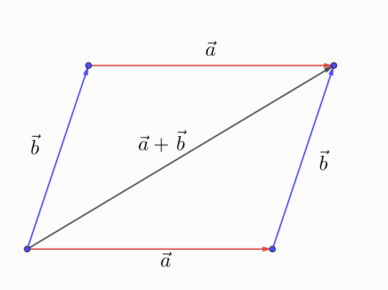
\includegraphics[width=0.4\textwidth]{images/pravilo_parallelogramma.png}
\end{center}

\begin{definition}
	\textit{Произведение вектора на число} $\overline{b} = \lambda\overline(a)$ $-$ вектор коллинеарный данному, а его модуль равен модулю данного вектора, умноженного на число. При этом
	\begin{enumerate}
		\item $\lambda = 0 \longrightarrow \overline{b} = \overline{0}$
		\item $\lambda < 0 \longrightarrow \overline{b}$ противоположно направлен $\overline{a}$
		\item $\lambda > 0 \longrightarrow \overline{b}$ сонаправлен $\overline{a}$
	\end{enumerate}
\end{definition}

\begin{definition}
	\textit{Разность векторов} определяется через операции сложения и умножения на число $\overline{a} - \overline{b} = \overline{a} + (-1)\overline{b}$.
\end{definition}

\textit{Свойства операций над векторами:}
\begin{enumerate}
	\item $\forall\overline{a},\overline{b}\tab\overline{a} + \overline{b} = \overline{b} + \overline{a}$
	\item $\forall\overline{a},\overline{b},\overline{c}\tab\overline{a} + (\overline{b} + \overline{c}) = (\overline{a} + \overline{b}) + \overline{c}$
	\item $\forall\overline{a}\tab\overline{a} + \overline{0} = \overline{a}$
	\item $\forall\overline{a}\tab\exists(-1)\overline{a} = -\overline{a}$ $-$ противоположный : $\overline{a} + (-\overline{a}) = \overline{0}$
	\item $\forall \alpha,\beta\in\R,\forall\overline{a}\tab(\alpha\beta)\overline{a}=\alpha(\beta\overline{a})$
	\item$\forall\overline{a}\tab1\cdot\overline{a}=\overline{a}$
	\item$\forall\alpha,\beta\in\R\tab(\alpha + \beta)\overline{a} = \alpha\overline{a}+\beta\overline{a}$
	\item$\forall\alpha\in\R,\forall\overline{a},\overline{b}\tab\alpha(\overline{a}+\overline{b})=\alpha\overline{a}+\alpha\overline{b}$
\end{enumerate}
\subsection{Линейная комбинация. Линейная зависимость и независимость}

\begin{definition}
	Если существует $\overline{a_1}$, ..., $\overline{a_n}$ и $\alpha_1$, ..., $\alpha_n$, то $\overline{b}=\alpha_1\overline{a_1}+...+\alpha_n\overline{a_n}$ $-$ $\textit{линейная комбинация}$. 
\end{definition}

Линейная комбинация называется $\textit{тривиальной}$, если все коэффициенты $\alpha_1=...=\alpha_n=0$, иначе $\textit{нетривиальной}$.

\begin{definition}
	Набор векторов $\overline{a_1}$, ..., $\overline{a_n}$ называют $\textit{линейно зависимым}$, если
	\begin{center}
		$\exists\alpha_1$, ..., $\alpha_n$ : $\alpha_1^2+...+\alpha_n^2 > 0$ : $\alpha_1\overline{a_1}+...+\alpha_n\overline{a_n} = \overline{0}$
	\end{center}
\end{definition}

\begin{definition}
	Набор векторов называется $\textit{линейно независимым}$, если только тривиальная комбинация дает нулевой вектор.
\end{definition}

\textit{Свойства:}

\begin{enumerate}
	\item если в наборе есть нулевой вектор, то этот набор линейно зависим
	\item если $\exists\overline{a_1}$, ..., $\overline{a_n}$ $-$ линейно зависимая комбинация, то $\forall\overline{b_1}$, ..., $\overline{b_m}}$, то набор $\overline{a_1}$, ..., $\overline{a_n}, \overline{b_1}$, ..., $\overline{b_m}$ $-$ линейно зависмый
	\item если набор линейно независим, то его любой непустой поднабор тоже линейно независим
	\begin{proof}
		Пусть этот поднабор линейно независим, но тогда по свойству 2 весь набор линейно зависм $\longrightarrow$ противоречие.
	\end{proof}
\end{enumerate}

\begin{theorem}
	Пусть $\overline{x}$ $-$ линейная комбинация, т.е. $\overline{x}=\alpha_1\overline{a_1}+...+\alpha_n\overline{a_n}$. Тогда разложение $\overline{x}$ единсьвенное $\longleftrightarrow$ $\overline{a_1}$, ..., $\overline{a_n}$ $-$ линейно независмый набор.
\end{theorem}

\begin{proof}
	\tab
	$\longrightarrow$\\
	Пусть существует
	\begin{center}
		$\overline{x}=\alpha_1\overline{a_1}+...+\alpha_n\overline{a_n}\tab(1)$\\
		$\overline{x}=\beta_1\overline{a_1}+...+\beta_n\overline{a_n}\tab(2)$
	\end{center}
	Вычтем (1) из (2) $\longrightarrow$ существует $\alpha_i\neq\beta_i$ $\longrightarrow$ нетривиальная $\longrightarrow$ противоречие.
	
	$\tab\longleftarrow$\\
	Пусть $\overline{a_1}$, ..., $\overline{a_n}$ - линейно зависим $\longrightarrow$ $\exists$нетривиальная линейная комбинация $\gamma_1\overline{a_1}$, ..., $\gamma_n\overline{a_n} = \overline{0}$\\
	
	$\overline{x} = \overline{x} + \overline{0} = (\alpha_1 + \gamma_1)\overline{a_1}+...+(\alpha_n + \gamma_n)\overline{a_n}$ $\longrightarrow$ разложение не единственно $\longrightarrow$ противоречие.
\end{proof}

\begin{theorem}[Критерий линейной зависимости]
	Набор из k > 1 элементов линейно зависим $\longleftrightarrow$ существует вектор набора, равный линейной комбинации остальных.
\end{theorem}
\begin{proof}
	$\tab\longrightarrow$\\
	Предположим, что $\overline{a_1}$, ..., $\overline{a_k}$ $-$ линейно зависима, тогда $\exists\alpha_1$, ..., $\alpha_k$ :  $\alpha_1^2+...+\alpha_k^2$ > 0, $\alpha_1\overline{a_1}+...+\alpha_k\overline{a_k}=\overline{0}$.\\
	Пусть $\alpha_1\neq0$ $\longrightarrow$ $\overline{a_1} = -\frac{\alpha_2}{\alpha_1}\overline{a_2}-...-\frac{\alpha_k}{\alpha_1}\overline{a_2}$ $-$ вектор $\overline{a_1}$ раскладывается по остальным векторам.
	
	$\tab\longleftarrow$\\
	Пусть $\overline{a_1} = p_2\overline{a_2}+...+p_k\overline{a_k}$, тогда коэффициент при $\overline{a_1}$ = 1 $\longrightarrow$ $1\cdot\overline{a_1}+(-p_2)\overline{a_2}+...+(-p_k)\overline{a_k}=\overline{0}$ $-$ нетривиальная комбинация $\longrightarrow$ линейно зависимая.
\end{proof}

\begin{corollary}
	Рассмотрим следствия 1 - 3 без доказательства, т.к. они очевидны.\\
	\begin{enumerate}
		\item нетривиальная комбинация векторов линейно независимого набора всегда не равна $\overline{0}$
		\item система из одно вектора линейно зависима $\longleftrightarrow$ этот вектор нулевой
		\item система из двух векторов линейно зависима $\longleftrightarrow$ эти векторв коллинеарны
		\item система из трех векторов линейно зависима $\longleftrightarrow$ эти векторы компланарны
		\begin{proof}
			Пусть $\overline{a}, \overline{b}, \overline{c}$ $-$ компланарны.
			\begin{enumerate}
				\item Пусть $\overline{a}$ и $\overline{b}$ $-$ коллинеарны $\longrightarrow$ из следствия 3 они линейно зависимы, а значит весь набор линейно зависим.
				\item Пусть эти векторы неколлинеарны, тогда по правилу параллелограмма $\exists\alpha, \beta$ : $\alpha\overline{a}+\beta\overline{b}=\overline{c}$
			\end{enumerate}
		\end{proof}
		
		\item система из четырех и более векторов линейно зависима всегда
		\begin{proof} Пусть даны векторы $\overline{a}, \overline{b}, \overline{c}, \overline{d}$.
			\begin{enumerate}
				\item Если есть нулевой вектор, то набор линейно завсимый
				\item если все векторы ненулевые
				\begin{enumerate}
					\item Если $\overline{a}, \overline{b}, \overline{c}$ $-$ компланарны, то из следствия 4 вся система линейно зависима
					\item Если $\overline{a}, \overline{b}, \overline{c}$ $-$ некомпланарны достаточно доказать, что $\overline{d}$ является их линейной комбинацией.\\
					Для этого построим плоскость, проходящую через векторы Если $\overline{a}, \overline{b}$C. Проведем через $\overline{d}$ вектор, параллельный $\overline{c}$ $-$ $\overline{c_1}$.
					\begin{center}
						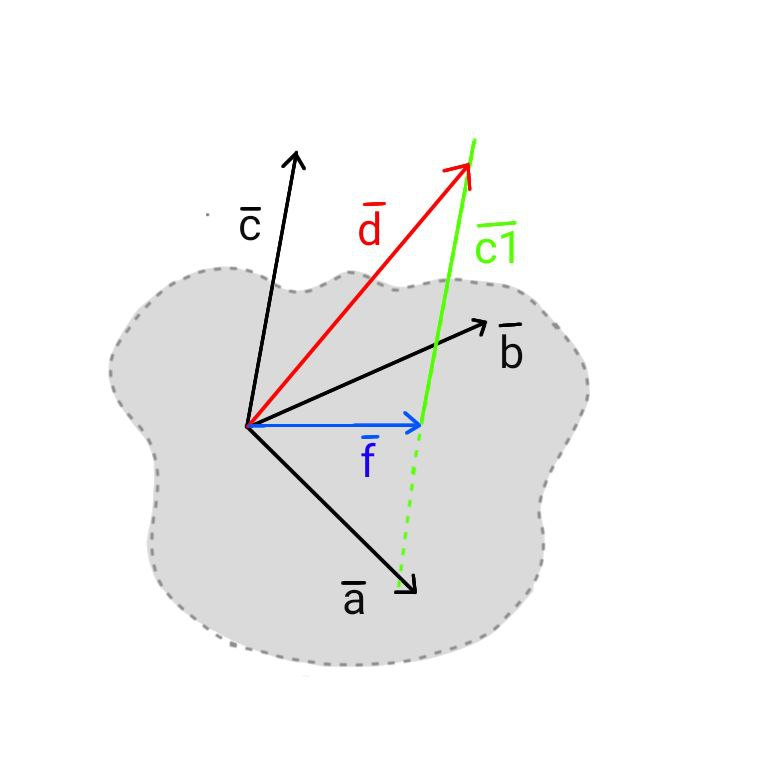
\includegraphics[width=0.4\textwidth]{images/5.jpeg}
					\end{center}
				\end{enumerate}
				$\overline{f}$ $-$ вектор к точке пересечения $\overline{c_1}$ с плоскостью. Т.к. Если $\overline{a}$ и $\overline{b}$ неколлинеарные, $\overline{f}$ можно разложить по ним:\\
				$\begin{cases}
					\overline{f} = \alpha\overline{a}+\beta\overline{b}\\
					\overline{c_1}=\gamma\overline{c}\\
				\end{cases}$ $\longrightarrow$ $\overline{d}=\overline{f}+\overline{c_1}= \alpha\overline{a}+\beta\overline{b}+\gamma\overline{c}$, значит $\overline{d}$ раскладывается по остальным векторам и система линейно зависимая.
			\end{enumerate}
		\end{proof}
		
	\end{enumerate}
\end{corollary}
